\documentclass[12pt,a4paper]{article}
\usepackage[utf8]{inputenc}
\usepackage{geometry}
\geometry{margin=1in}
\usepackage{enumitem}
\usepackage{hyperref}
\usepackage{graphicx}
\usepackage{float}

\begin{document}

% -------------------------------
% SIMPLE HEADER
% -------------------------------
\begin{center}
    {\Huge \textbf{AI Customer Support Egyptian Service}}\\[0.5cm]
    {\Large Graduation Project Proposal for Sponsorship}\\[0.3cm]
    {\large Faculty of Computer Science, Benha National University}\\[0.3cm]
    {\large Academic Year: 2025–2026}\\[1cm]
\end{center}

% -------------------------------
\section*{1. Idea Description}
Our project is an AI-powered, customizable Arabic "Egyptian" customer support platform designed to help SMEs automate their customer service across channels like WhatsApp, Messenger, and web platforms by integrating our service.

\textbf{Main Features:}
\begin{itemize}[noitemsep]
    \item Understanding of the Arabic dialect of Egypt.
    \item Customization \& rule for answers
    \item Text support
    \item Voice support (speech-to-text \& text-to-speech).
    \item Real-time emotion detection.
    \item Multi-intent handling.
    \item Integrations: WhatsApp, Messenger, Websites, Apps.
\end{itemize}

% -------------------------------
\section*{2. Mini Business Plan}
\textbf{Problem:} Egyptian SMEs struggle to deliver 24/7 customer support. They face repetitive questions, missed 
messages, and slow response times. Existing chatbot platforms are either too expensive, rigid, or 
lack proper Egyptian Arabic support. \\

\textbf{Solution:} An AI-powered, customizable customer support system that integrates with WhatsApp, 
Messenger, and web. It supports Egyptian Arabic, voice, and emotion detection, and gives 
businesses control over customization. \\

\textbf{Target Customers:} SMEs in Egypt and the MENA region—especially those relying on social media and web 
platforms to interact with customers. \\

\textbf{Why It Matters:} This makes small businesses more competitive, improves customer satisfaction, reduces manual 
workload, and provides a localized solution that global players don't offer. \\

% -------------------------------
\newpage
\section*{3. Prototype - System Analysis}
We are currently in the system analysis phase. The following diagrams represent our vision and planned design:  
\begin{center}
    \includegraphics[width=0.5\linewidth]{AI layer.png}\\
    \textbf{1-Figure:} AI Layer Flow Chart (MVP Implementation)
\end{center}

\begin{center}
    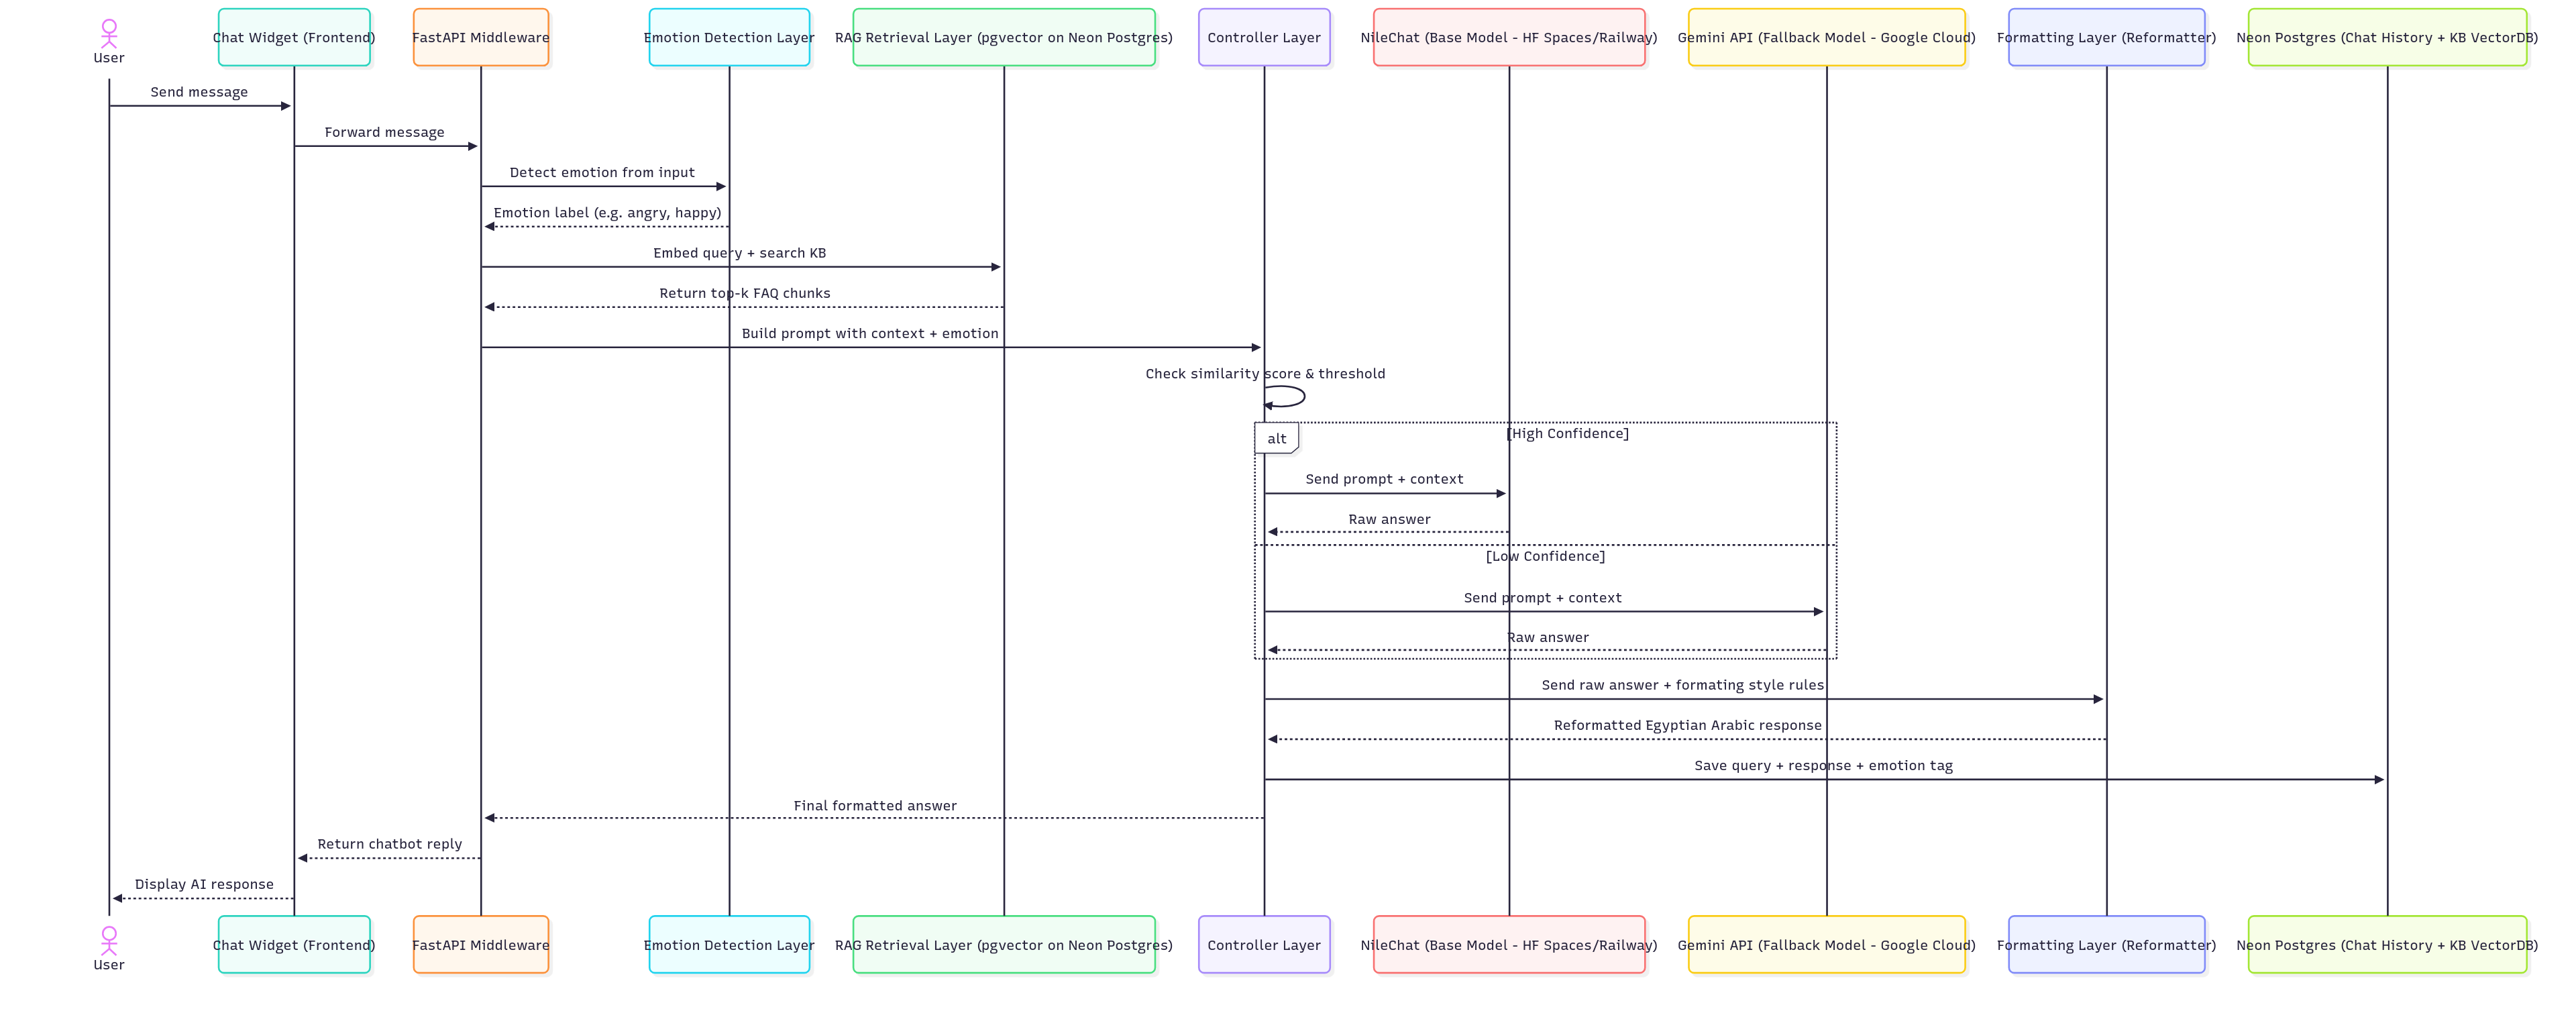
\includegraphics[width=1\linewidth]{example for sequence diagram.png}
    \\ Sequence Diagram For User(MVP Implementation)
\end{center}
\begin{center}
    \includegraphics[width=1\linewidth]{sequencebusiness.png}
    \\ Sequence Diagram For business Admin (MVP Implementation)
\end{center}
% Placeholder for Use Case Diagram
\begin{center}
     \includegraphics[width=1\linewidth]{Usecase.png}
   \\ Use Case Diagram (MVP Implementation)
\end{center}

% Placeholder for DFD Level 0
\begin{center}
      \includegraphics[width=1\linewidth]{DFDlevel0.png}
    \\ DFD level 0 "context" Diagram (MVP Implementation)
\end{center}

% % Placeholder for DFD Level 1
\begin{center}
    \includegraphics[width=0.8\linewidth]{DFD level1.png}
    \\ DFD level 1 Diagram (MVP Implementation)
\end{center}

\begin{center}
    \includegraphics[width=0.8\linewidth]{DFD level2.png}
    \\ DFD level 2 Diagram (MVP Implementation)
\end{center}

\newpage
% -------------------------------
\section*{4. Technology Stack \& Roadmap Until Graduation}
\textbf{Technology Stack:}
\begin{itemize}
    \item Backend: Python + FastAPI
    \item Frontend: React.js (Chat Widget + Admin Dashboard)
    \item Database: PostgreSQL with Vector Extension "NeonDB"
    \item AI/NLP: NileChat, Gemini or Qwen, Whisper or Sada, HuggingFace APIs, LangChain
    \item Deployment \& DevOps: Docker, Railway, GitHub CI/CD
    \item Integrations: WhatsApp Business API, Facebook API, Instagram API, web widget
\end{itemize}

\subsection{Phases and Roadmap}

The project will be executed across two academic terms.  
The first term focuses on building and delivering the initial MVP, while the second term extends the system with additional features and demonstrations.

\subsubsection*{Term 1: MVP Development}
\begin{enumerate}[leftmargin=*]
    \item \textbf{System Analysis \& Prototype Design}  
    -- Gather detailed requirements, refine system analysis, and design a low-fidelity prototype (wireframes, mockups).  
    -- Validate requirements with supervisor feedback.  

    \item \textbf{MVP Implementation}  
    -- Develop the core backend (FastAPI + PostgreSQL) and frontend chat widget, sample dashboard (React).  
    -- Integrate the AI models (NileChat \& Gemini API or other) with prompt engineering.  
    -- Add initial emotion detection, RAG integration, and formatting layers.  
    -- Implement company authentication and chat history storage.  

    \item \textbf{Testing the MVP}  
    -- Internal testing of core flows (chatbot answering FAQs, emotion detection, RAG retrieval).  
    -- Fix bugs and validate performance with simple datasets.  

    \item \textbf{Deployment of MVP}  
    -- Deploy on cloud (Railway / Docker).  
    -- First demo at the end of Term 1 showing a functional text-based MVP.  
\end{enumerate}

\subsubsection*{Term 2: Extended Development and Demo}
\begin{enumerate}[leftmargin=*]
    \item \textbf{Feature Expansion}  
    -- Add advanced features: advanced emotion detection, more details on admin dashboard, voice support (Whisper + TTS), and expanded customization options for businesses.  
    -- Integrate with WhatsApp, Facebook, and Instagram APIs.  

    \item \textbf{Testing and Refinement}  
    -- Conduct user testing with SMEs to evaluate new features.  
    -- Measure accuracy, response quality, and user satisfaction.  

    \item \textbf{Deployment of Enhanced Version}  
    -- Deploy extended version with added features.  
    -- Optimize performance and ensure scalability.  

    \item \textbf{Final Demonstration}  
    -- Deliver a comprehensive demo including both the initial MVP and extended features.  
\end{enumerate}

\subsubsection*{Summary Timeline}
\begin{itemize}[leftmargin=*]
    \item \textbf{Weeks 1--3 (Term 1):} System analysis, prototype design, infrastructure setup.  
    \item \textbf{Weeks 4--8 (Term 1):} MVP development (backend, frontend, AI integration, emotion detection, and RAG).  
    \item \textbf{Weeks 9--12 (Term 1):} Internal testing, bug fixing, and initial demo deployment.  
    \item \textbf{Term 2 (Months 5--8):} Feature expansion (dashboard, voice, advanced integrations), second round of testing, deployment, and final demo.  
\end{itemize}

% -------------------------------
\section*{5.Team Roles \& Info}
\subsection*{Team Roles}
\begin{itemize}[leftmargin=*]
    \item \textbf{Backend Developers (3):} Responsible for core APIs, databases, pipelines, and also assisting the AI engineer.  
    \item \textbf{Frontend Developers (2):} Handle UI/UX, build the chatbot widget and dashboard.  
    \item \textbf{AI Engineer (1):} Focused on AI/NLP integration, RAG, emotion detection, and orchestration layers.  
    \item \textbf{DevOps:} Tasks (containerization, CI/CD, monitoring) will be handled by the backend team.  
\end{itemize}

\subsection*{Team Information}

\textbf{1. Ahmed Ehab Elattar – Project Manager \& Backend Developer}  
\begin{itemize}
    \item Email: \href{mailto:ahmeddelattarr@outlook.com}{ahmeddelattarr@outlook.com}
    \item LinkedIn: \href{https://www.linkedin.com/in/ahmedelattar-tr}{linkedin.com/in/ahmedelattar-tr}
    \item GitHub: \href{https://github.com/ahmeddelattarr}{github.com/ahmeddelattarr}
    \item Portfolio: \href{https://www.ahmedelattar.tech}{ahmedelattar.tech}
    \item CV: \href{https://www.ahmedelattar.tech/resume.pdf}{Ahmed Resume PDF}
    \item Specialization: Backend, Python, FastAPI, System Architecture, Project Management, AI/NLP, DevOps, PostgreSQL
\end{itemize}

\textbf{2. Bassant Hossam Salah Eldeen – Backend Developer}  
\begin{itemize}
    \item Email: \href{mailto:bassanthosamm1@outlook.com}{bassanthosamm1@outlook.com}
    \item LinkedIn: \href{https://www.linkedin.com/in/bassant-hossam-5a4177264}{linkedin.com/in/bassant-hossam}
    \item GitHub: \href{https://github.com/Bassanthossamxx}{github.com/bassanthossamxx}
    \item Portfolio: \href{https://bassant-portfolio.vercel.app}{bassant-portfolio.vercel.app}
    \item CV: \href{https://bassant-portfolio.vercel.app/assets/Bassant_Hossam_CV.pdf}{Bassant Resume PDF}
    \item Specialization: Backend, Python, FastAPI, PostgreSQL, AI/NLP, DevOps
\end{itemize}

\textbf{3. Eyad Hesham – Frontend Developer}  
\begin{itemize}
    \item Email: \href{mailto:eyadtalha04@gmail.com}{eyadtalha04@gmail.com}
    \item LinkedIn: \href{https://www.linkedin.com/in/eyadhesham}{linkedin.com/in/eyadhesham}
    \item GitHub: \href{https://github.com/EyadTalha}{github.com/EyadTalha}
    \item CV: \href{https://drive.google.com/file/d/1gIWggXZtLGkVX9wEBdzE1umS1afZiNBz/view?usp=sharing}{Eyad Resume PDF}
    \item Specialization: UI/UX, React.js, Security Implementation, DevOps
\end{itemize}

\textbf{4. Shahda Mohamed Abotalb – Backend Developer}  
\begin{itemize}
    \item Email: \href{mailto:shahdamohamedabotalb@gmail.com}{shahdamohamedabotalb@gmail.com}
    \item LinkedIn: \href{https://www.linkedin.com/in/shahda-mohamed-178537280}{linkedin.com/in/shahda-mohamed}
    \item Portfolio: \href{https://shahdamohamed.github.io/my-website}{shahdamohamed.github.io/my-website}
    \item GitHub: \href{https://github.com/shahdamohamed}{github.com/shahdamohamed}
    \item CV: \href{https://shahdamohamed.github.io/my-website/assets/resume.pdf}{Shahda Resume PDF}
    \item Specialization: Backend, Python, FastAPI, DevOps
\end{itemize}

\textbf{5. Zead Wael – Frontend Developer}  
\begin{itemize}
    \item Email: \href{mailto:zeyadwaelcs@gmail.com}{zeyadwaelcs@gmail.com}
    \item LinkedIn: \href{https://www.linkedin.com/in/zead-wael}{linkedin.com/in/zead-wael}
    \item GitHub: \href{https://github.com/ZeadWael}{github.com/ZeadWael}
    \item CV: \href{https://drive.google.com/drive/folders/1mSTjcvvaDnJasdTxr2x36CddeTrQR5dQ?usp=sharing}{Zead Resume PDF}
    \item Specialization: UI/UX, React.js, Pen-testing, Security Implementation, DevOps
\end{itemize}

\textbf{6. Toni Ihab – AI Specialist}  
\begin{itemize}
    \item Email: \href{mailto:tony0100512@cs.bnu.edu.eg}{tony0100512@cs.bnu.edu.eg}
    \item LinkedIn: \href{https://www.linkedin.com/in/toni-ihab/}{linkedin.com/in/toni-ihab}
    \item GitHub: \href{https://github.com/tokihab}{github.com/tokihab}
    \item Specialization: AI, ML, NLP, Pen-testing, DevOps 
\end{itemize}

% -------------------------------
\section*{6. Support Required from Sponsor}
\begin{itemize}
    \item Mentorship, especially in AI part and integration.
    \item Design Support (UI/UX improvement).
    \item Partnerships if valid with SMEs to pilot MVP.
    \item Funding (hosting, AI APIs, deployment costs).
\end{itemize}

% -------------------------------
\section*{7. Expected Cost}

For the MVP phase, most components will rely on free or student plans:

\begin{itemize}[leftmargin=1.2em]
    \item \textbf{Domain:} Student or free domain plan, estimated at \textasciitilde\$1/month if upgraded.
    \item \textbf{Deployment:} Free hosting tiers (Railway/Render/Koyeb). Upgrade to hobby plan (\$7--\$10/month) only if traffic grows.
    \item \textbf{Database:} NeonDB Free tier (191 compute hours, 0.5 GB storage). Launch plan starts at \$19/month if traffic increases.
    \item \textbf{Frontend:} Free tier (Vercel/Netlify). Upgrade later if usage exceeds limits (\$20/month).
    \item \textbf{APIs and AI Models:} 
    \begin{itemize}
        \item \textbf{NileChat:} Self-hosted, free aside from GPU time (estimate \$10--\$15/month for light usage).
        \item \textbf{Gemini API:} Free student plan available (Google AI Pro). Paid usage \textasciitilde\$5--\$10/month for fallback calls.
    \end{itemize}
\end{itemize}

\textbf{Total Expected Monthly Cost:}  
\begin{itemize}
    \item Low traffic (using free/student tiers): \textasciitilde\$20/month.
    \item Moderate traffic (hobby + light API usage): \textasciitilde\$35--\$50/month.
    \item Heavy GPU/API usage: up to \textasciitilde\$60--\$70/month.
\end{itemize}

\end{document}
